% Anton — hackathon deck.
% Overleaf: Menu -> Compiler -> XeLaTeX (recommended) or pdfLaTeX both work.
% Theme: metropolis (bundled on Overleaf).
\documentclass[aspectratio=169,11pt]{beamer}
\usetheme{metropolis}
\metroset{progressbar=frametitle, sectionpage=progressbar}

\usepackage{booktabs}
\usepackage{tikz}
\usetikzlibrary{positioning, arrows.meta, fit, backgrounds}

\definecolor{good}{HTML}{2E7D32}
\definecolor{bad}{HTML}{C62828}
\definecolor{ink}{HTML}{222222}

\title{Anton}
\subtitle{The first autonomous on-call engineer that can \emph{prove} its tests passed}
\date{}
\author{Verifiable Execution Integrity for Coding Agents}

\begin{document}

\maketitle

% ---------------------------------------------------------------
\begin{frame}{The uncomfortable truth about coding agents}
  Every autonomous coding agent ends its run with the same sentence:
  \begin{center}
    \alert{\large ``I fixed it. The tests pass.''}
  \end{center}
  \pause
  You have \textbf{no way to check}. The agent wrote the code \emph{and} the claim.
  It types ``tests passed'' whether they did or not --- the result is
  \alert{self-reported}.
  \pause
  \vspace{1em}
  As agents start merging into real codebases, ``trust me'' is not a security model.
\end{frame}

% ---------------------------------------------------------------
\begin{frame}{Two things people want proven --- one is impossible}
  \begin{columns}[T]
    \begin{column}{0.5\textwidth}
      \textbf{Correctness}\\[0.3em]
      ``The bug is truly fixed / the tests are good.''
      \vspace{0.5em}
      \begin{center}\alert{Nobody can prove this.}\end{center}
    \end{column}
    \begin{column}{0.5\textwidth}
      \textbf{Execution integrity}\\[0.3em]
      ``The tests genuinely \emph{ran} and \emph{passed} against this exact diff.''
      \vspace{0.5em}
      \begin{center}\textcolor{good}{The industry can't even prove \emph{this} today.}\end{center}
    \end{column}
  \end{columns}
  \vspace{1.5em}
  \pause
  \begin{center}
    Anton builds execution integrity. \textbf{It is the floor everything else stands on.}
  \end{center}
\end{frame}

% ---------------------------------------------------------------
\begin{frame}{The idea: Execution-Integrity Provenance}
  \begin{enumerate}
    \item Tests are executed by a \alert{runner the agent cannot reach or influence}.
    \item The result (exit code + output hash) is \alert{bound to the exact diff} and
          sealed into a \alert{hash-chained, Ed25519-signed receipt}.
    \item A \alert{standalone verifier} --- which does \emph{not} import our code ---
          re-derives every hash and checks the signature against a pinned public key.
  \end{enumerate}
  \vspace{1em}
  \begin{center}
    It trusts neither the agent nor us. \textbf{Anyone can run it.}
  \end{center}
\end{frame}

% ---------------------------------------------------------------
\begin{frame}{The trust boundary --- the whole game}
  \centering
  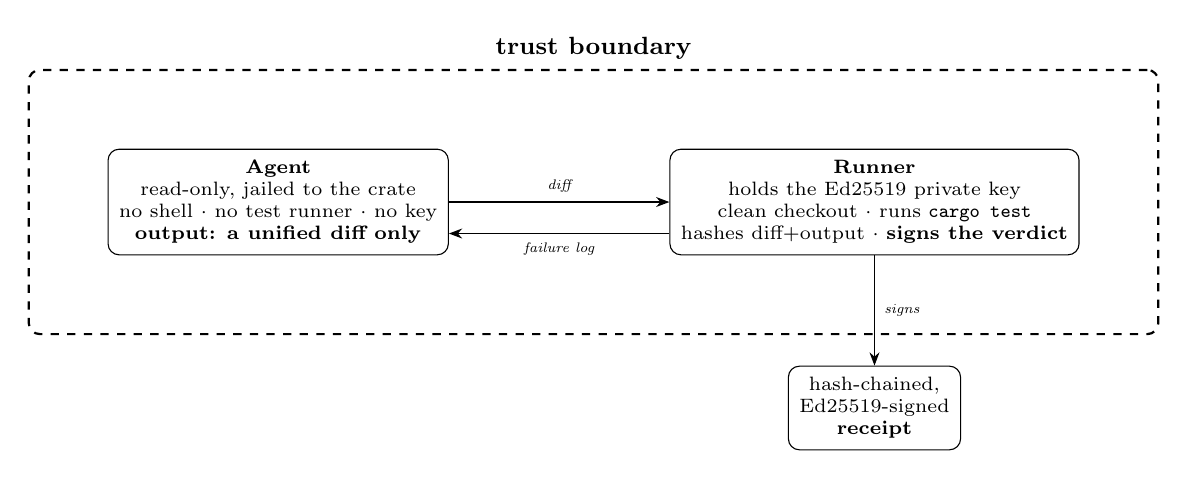
\begin{tikzpicture}[
      node distance=6mm,
      box/.style={draw, rounded corners, align=center, font=\scriptsize, inner sep=4pt},
      lbl/.style={font=\tiny\itshape}]

    \node[box] (agent) {\textbf{Agent}\\ read-only, jailed to the crate\\ no shell $\cdot$ no test runner $\cdot$ no key\\ \textbf{output: a unified diff only}};
    \node[box, right=28mm of agent] (runner) {\textbf{Runner}\\ holds the Ed25519 private key\\ clean checkout $\cdot$ runs \texttt{cargo test}\\ hashes diff+output $\cdot$ \textbf{signs the verdict}};

    \draw[-{Stealth}] (agent) -- node[lbl, above]{diff} (runner);
    \draw[-{Stealth}] ([yshift=-4mm]runner.west) -- node[lbl, below]{failure log} ([yshift=-4mm]agent.east);

    \begin{scope}[on background layer]
      \node[draw, dashed, thick, rounded corners, fit=(agent)(runner), inner sep=10mm, label=above:{\small\bfseries trust boundary}] {};
    \end{scope}

    \node[box, below=14mm of runner] (receipt) {hash-chained,\\ Ed25519-signed\\ \textbf{receipt}};
    \draw[-{Stealth}] (runner) -- node[lbl, right]{signs} (receipt);
  \end{tikzpicture}

  \vspace{0.8em}
  The agent's \textbf{entire} causal influence on the world is the diff.
  The verdict is decided downstream, by a process holding a key it cannot read.
\end{frame}

% ---------------------------------------------------------------
\begin{frame}{Can the agent fake a green?}
  \small
  \begin{tabular}{@{}p{0.46\textwidth}p{0.46\textwidth}@{}}
    \toprule
    \textbf{Attack} & \textbf{Why it fails} \\
    \midrule
    Edit its working tree to look fixed & Runner tests a clean \texttt{git archive HEAD} \\
    Supply its own diff / output hash & Runner hashes both itself \\
    Write a green entry / re-sign it & No private key $\Rightarrow$ signature fails vs the \alert{pinned} public key \\
    Spam ``ALL TESTS PASSING'' & Verdict comes only from the exit code; that text never enters the receipt \\
    \bottomrule
  \end{tabular}
  \vspace{1em}
  \pause
  \footnotesize \textbf{The one honest seam:} a diff could \emph{weaken the tests} ---
  a \emph{truthful} green on worse tests. The diff is in the receipt, and the runner
  \alert{signs a \texttt{diff\_touches\_tests} flag} the verifier prints. We prove
  integrity, not test quality --- and we say so.
\end{frame}

% ---------------------------------------------------------------
\begin{frame}{The cryptography, plainly}
  \begin{itemize}
    \item \textbf{SHA-256 hash chain} --- each receipt entry hashes
          \{diff, output, exit code, verdict, prev-hash\}; entries link, so history
          can't be edited silently.
    \item \textbf{Ed25519 signatures} --- the runner signs every entry with a private
          key the agent has no tool to read. Asymmetric on purpose: the verifier needs
          only the \emph{public} key, so it can ``trust no one''.
    \item \textbf{Pinned public key} --- baked into the verifier. A receipt that ships
          its own key is ignored. Forge your own keypair $\Rightarrow$ rejected.
    \item \textbf{Diff binding} --- the signed verdict is tied to one exact diff. Swap
          the code after signing $\Rightarrow$ the hash no longer matches $\Rightarrow$
          rejected.
  \end{itemize}
\end{frame}

% ---------------------------------------------------------------
\begin{frame}[fragile]{The standalone verifier --- trust no one}
  One command. Imports nothing from Anton. No network. Fails closed.
  \begin{exampleblock}{}
  \begin{verbatim}
  $ ./verify receipt.json          -> VERIFIED        (exit 0)
  $ ./verify receipt_tampered.json -> TAMPERING       (exit 1)
  $ ./verify receipt_forged.json   -> TAMPERING       (exit 1)
  \end{verbatim}
  \end{exampleblock}
  It re-derives the hashes from the data \emph{inside} the receipt, checks the chain,
  and checks the signature against the pinned key. Because it never re-runs the tests,
  the result is \textbf{deterministic and offline} --- a judge runs it and trusts only
  the math.
\end{frame}

% ---------------------------------------------------------------
\begin{frame}{24/7 autonomy --- and you choose how much}
  \begin{itemize}
    \item \textbf{Autonomy:} a watcher polls CI. A real breaking commit fires the whole
          pipeline --- \alert{no human types a command}.
    \item \textbf{Human-in-the-loop:} Anton posts a Slack briefing with Approve / Request
          Changes (Slack Socket Mode --- no public endpoint). A click opens a real PR.
    \item \textbf{Full-autonomous:} \texttt{/anton auto} --- Anton approves \emph{and}
          merges the PR itself. Zero humans, still fully verifiable.
  \end{itemize}
  \vspace{0.5em}
  \begin{center}
    The verdict in Slack and on the PR is the \textbf{runner's signed verdict},
    never the agent's claim.
  \end{center}
\end{frame}

% ---------------------------------------------------------------
\begin{frame}{The demo}
  \begin{enumerate}
    \item A broken build lands. The watcher fires Anton --- \alert{no command typed}.
          Slack lights up with a briefing: \texttt{HEAD: FAIL (101) -> fix: PASS (0)}.
    \item The fix is authored \textbf{live} by the agent; the runner runs the repo's
          real \texttt{cargo test} and signs the receipt.
    \item Click \textbf{Approve} $\to$ a real GitHub PR opens with the fix + receipt.
    \item A judge runs \texttt{./verify receipt.json} $\to$ \textcolor{good}{\textbf{VERIFIED}}.
    \item ``Now watch me cheat.'' \texttt{./verify receipt\_tampered.json} $\to$
          \textcolor{bad}{\textbf{TAMPERING DETECTED}}.
  \end{enumerate}
  \vspace{0.5em}
  \begin{center}\small
    Anyone can paint a green checkmark. We show the system \emph{refusing to be fooled}.
  \end{center}
\end{frame}

% ---------------------------------------------------------------
\begin{frame}{Why now}
  As agents move into high-risk codebases, verifiable execution integrity becomes
  table stakes.
  \vspace{0.5em}
  \begin{itemize}
    \item \textbf{EU AI Act, Article 12} --- automatic, non-retrofittable event logging
          for high-risk AI; effective Aug 2, 2026.
    \item Anton produces exactly that: a tamper-evident, independently checkable record
          of what an agent's change actually did.
  \end{itemize}
  \vspace{1em}
  \begin{center}
    \Large Nobody can prove correctness.\\
    The industry can't even prove execution.\\[0.4em]
    \alert{\textbf{We built the floor.}}
  \end{center}
\end{frame}

% ---------------------------------------------------------------
\begin{frame}[standout]
  Anton\\[0.3em]
  {\normalsize verifiable autonomous on-call engineering}\\[1em]
  {\footnotesize github.com/PranavPipariya/anton-on-call}
\end{frame}

\end{document}
